%
%	Use lualatex
%
% !TEX TS-program = LuaLaTeX
%
%	To get overleaf.com to use lualatex see
%	https://www.overleaf.com/learn/how-to/Changing_compiler.
%	Basically, change the compiler in Settings.
%
\documentclass{article}
%
%
%	LaTeX template
%
%	David Meyer
%	dmm613@gmail.com
%	08 Oct 2023
%
%
%   get various packages
%
\usepackage[margin=1.0in]{geometry}                                     % adjust margins
\geometry{letterpaper}                                                  % or a4paper or a5paper or ... 
\usepackage{url}                                                        % need this to use URLs in bibtex
\usepackage{setspace}                                                   % need this for \setstrech{...}
\usepackage{scrextend}                                                  % need this for addmargin
\usepackage[export]{adjustbox}                                          % need this to get frame for includegraphics
%
%   tikz et al
%
\usepackage{tikz}
\tikzset{>=latex}                                                       % default to LaTeX arrow head
\usetikzlibrary{calc,patterns,angles,quotes,shapes,math,decorations,
                through,intersections,lindenmayersystems,backgrounds,
                hobby,matrix}
\usepackage{tikz-cd}
\tikzcdset{every arrow/.append style={-latex}}							% commutative diagrams
\usepackage{circuitikz}                                                 % draw circuits    
\usepackage{pgfplots}
%
%	more math stuff
%
\usepackage{amsmath,amsfonts,amssymb,amsthm}
\usepackage{bm}
\usepackage{mathtools}
\usepackage{commath}                                                    % get \norm{x}
\usepackage{fixmath}                                                    % get \mathbold
\usepackage{gensymb}                                                    % get \degree
\usepackage{mathrsfs}
\usepackage{hyperref}
\usepackage{subcaption}
\usepackage{authblk}													% comment out if using beamer (stops \author{} from working in beamer)
\usepackage{graphicx}
\usepackage{hyperref}
\usepackage{alltt}
\usepackage{xcolor}
\usepackage{colortbl}													% \rowcolor{yellow!75} etc
\usepackage{float}
\usepackage{braket}
\usepackage{siunitx}
\usepackage{relsize}
\usepackage{multirow}
\usepackage{esvect}
\usepackage{enumitem}													% use characters instead of numbers in enumerate
\usepackage{changepage}													% needed for \begin{adjustwidth}{-3.25em}{-2.0em} (left justify)
\usepackage{bigints}
\usepackage{multirow}													% \multirow and \multicolumn
\usepackage{enumitem}													% change bullets in \begin{enumerate}
%
%	lualatex
%
%	Put this before \documentclass
%
%	!TEX TS-program = LuaLaTeX
%
%
\usepackage{luatex85,luamplib}
\mplibnumbersystem{double}
\mplibtextextlabel{enable}
%
%
%
%	Describe floating point parameters, \fpeval
%
\ExplSyntaxOn
\cs_set_eq:NN \fpeval \fp_eval:n
\ExplSyntaxOff
%
%	Get the x and y components out of a coordinate, e.g.
%
%	\coordinate (EP) at (8,5);
%	\gettikzxy{(EP)}{\slopex}{\slopey}
%
\makeatletter
\newcommand{\gettikzxy}[3]{%
  \tikz@scan@one@point\pgfutil@firstofone#1\relax
  \edef#2{\the\pgf@x}%
  \edef#3{\the\pgf@y}%
}
\makeatother
%
%
%	Watermarks
%
% \usepackage{draftwatermark}
% \SetWatermarkText{Draft}
% \SetWatermarkScale{5}
% \SetWatermarkLightness {0.9} 
% \SetWatermarkColor[rgb]{0.7,0,0}
%
%
%	theorems, definitions, etc
%
\theoremstyle{definition}
\newtheorem{theorem}{Theorem}[section]
\newtheorem{definition}{Definition}[section]
\newtheorem{proposition}{Proposition}[section]
\newtheorem{lemma}{Lemma}[section]
\newtheorem{example}{Example}[section]
\newtheorem{remark}{Remark}[section]
\newtheorem{notation}{Notation}[section]
%
%	For drawing matrix products 
%
\newcommand*{\vertbar}{\rule[-1ex]{0.5pt}{2.5ex}}
\newcommand*{\horzbar}{\rule[.5ex]{2.5ex}{0.5pt}}

%
%	The following code allows you to do
%
%	\begin{bmatrix}[r] (or [c] or [l])
%
\makeatletter
\renewcommand*\env@matrix[1][c]{\hskip -\arraycolsep
  \let\@ifnextchar\new@ifnextchar
  \array{*\c@MaxMatrixCols #1}}
\makeatother
%
%	make \arg{min,max}_{n \to \infty} work nicely
%
\newcommand{\argmax}{\operatornamewithlimits{argmax}}
\newcommand{\argmin}{\operatornamewithlimits{argmin}}
%
%	handy commands
%
\newcommand*{\Scale}[2][4]{\scalebox{#1}{$#2$}}
\DeclareMathOperator{\E}{\mathbb{E}}
\DeclareMathOperator{\bda}{\Big \downarrow}						% big down arrow
\newcommand{\veq}{\mathrel{\rotatebox{90}{$=$}}}
%
%	Title, author and date
%
\title{Christmastime is Christmas Math Time!}
\author{David Meyer \\ \href{mailto:dmm613@gmail.com}
                            {dmm613@gmail.com}}
\date{Last Update: \today \\
	 {\vspace{1.00mm} \small Initial Version: September 20, 2020}}
%
%
%
\begin{document}
\maketitle
% \tableofcontents

%
%
%
\section {Introduction}

There are all kinds of interesting mathematics associated
with Christmas. This note outlines a few examples, starting
with The Infinite Gift and Gabriel's Horn.
%
%
%
\section{The Infinite Gift and Gabriel's Horn}
Analytic geometry is populated by all kinds of crazy
objects. Being that it is Christmastime (and therefore 
Christmas Math Time!) please check out the paradoxical 
object shown in Figure \ref{fig:infinite_gift}. This 
object is sometimes known as The Infinite Gift.


\medskip
\bigskip
\begin{figure} [H]
\center{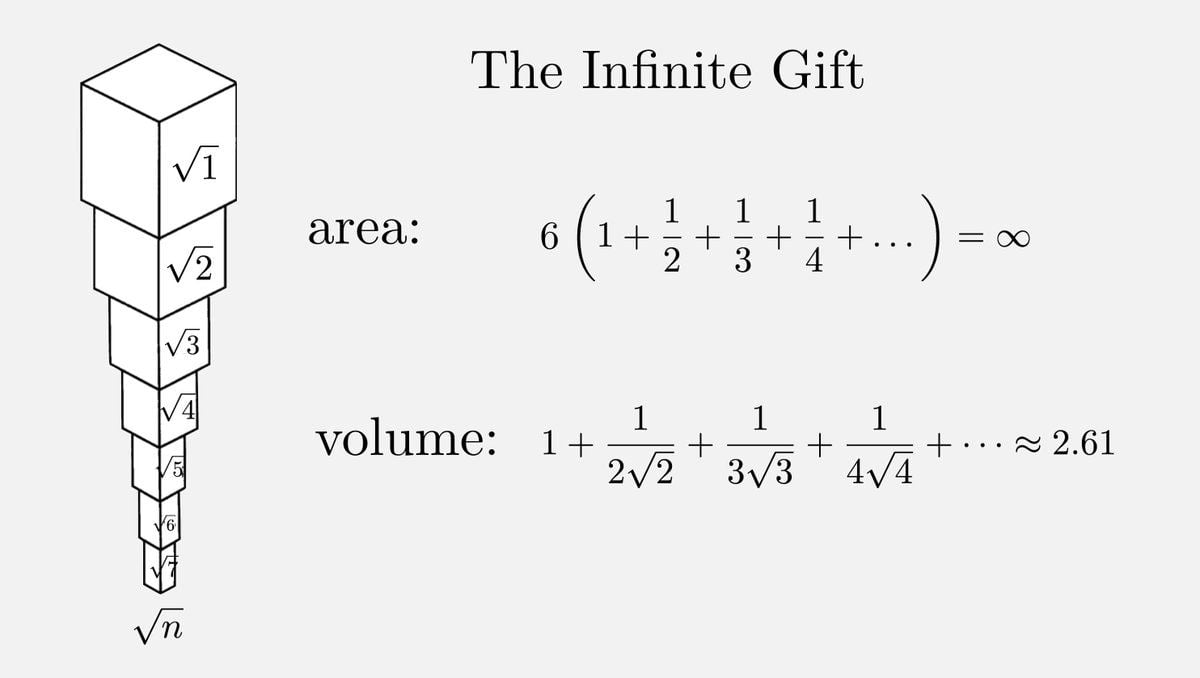
\includegraphics[frame, scale=0.25] {images/infinite_gift.jpg}}
\caption{The Infinite Gift}
\label{fig:infinite_gift}
\end{figure}

\bigskip
{\setstretch{1.50}
\noindent
In the Infinite Gift the length of the side of the $n^{th}$ box
is $\frac{1}{\sqrt{n}}$ so the area of a side of the $n^{th}$ box
is ${\left ( \frac{1}{\sqrt{n}}\right ) }^2 = \frac{1}{n}$.
Since a box has 6 sides the surface area of the $n^{th}$ box is
$6 * \frac{1}{n}$. Then what you find is that in the limit (as $n
\to \infty$) the Infinite Gift has infinite surface area but
finite volume!  \par}


\bigskip
\noindent
Interesting aside: In the limit the area of the 
Infinite Gift equals 6 times the harmonic series
(which we know diverges \cite{wiki:harmonic}).


\bigskip
\noindent
The continuous version of this object is known as Gabriel's Horn
(aka Torricelli’s Trumpet) \cite{wolfram:gabriels_horn}, which is
shown in Figure \ref{fig:gabriels_horn}.

\bigskip
\begin{figure} [H]
\center{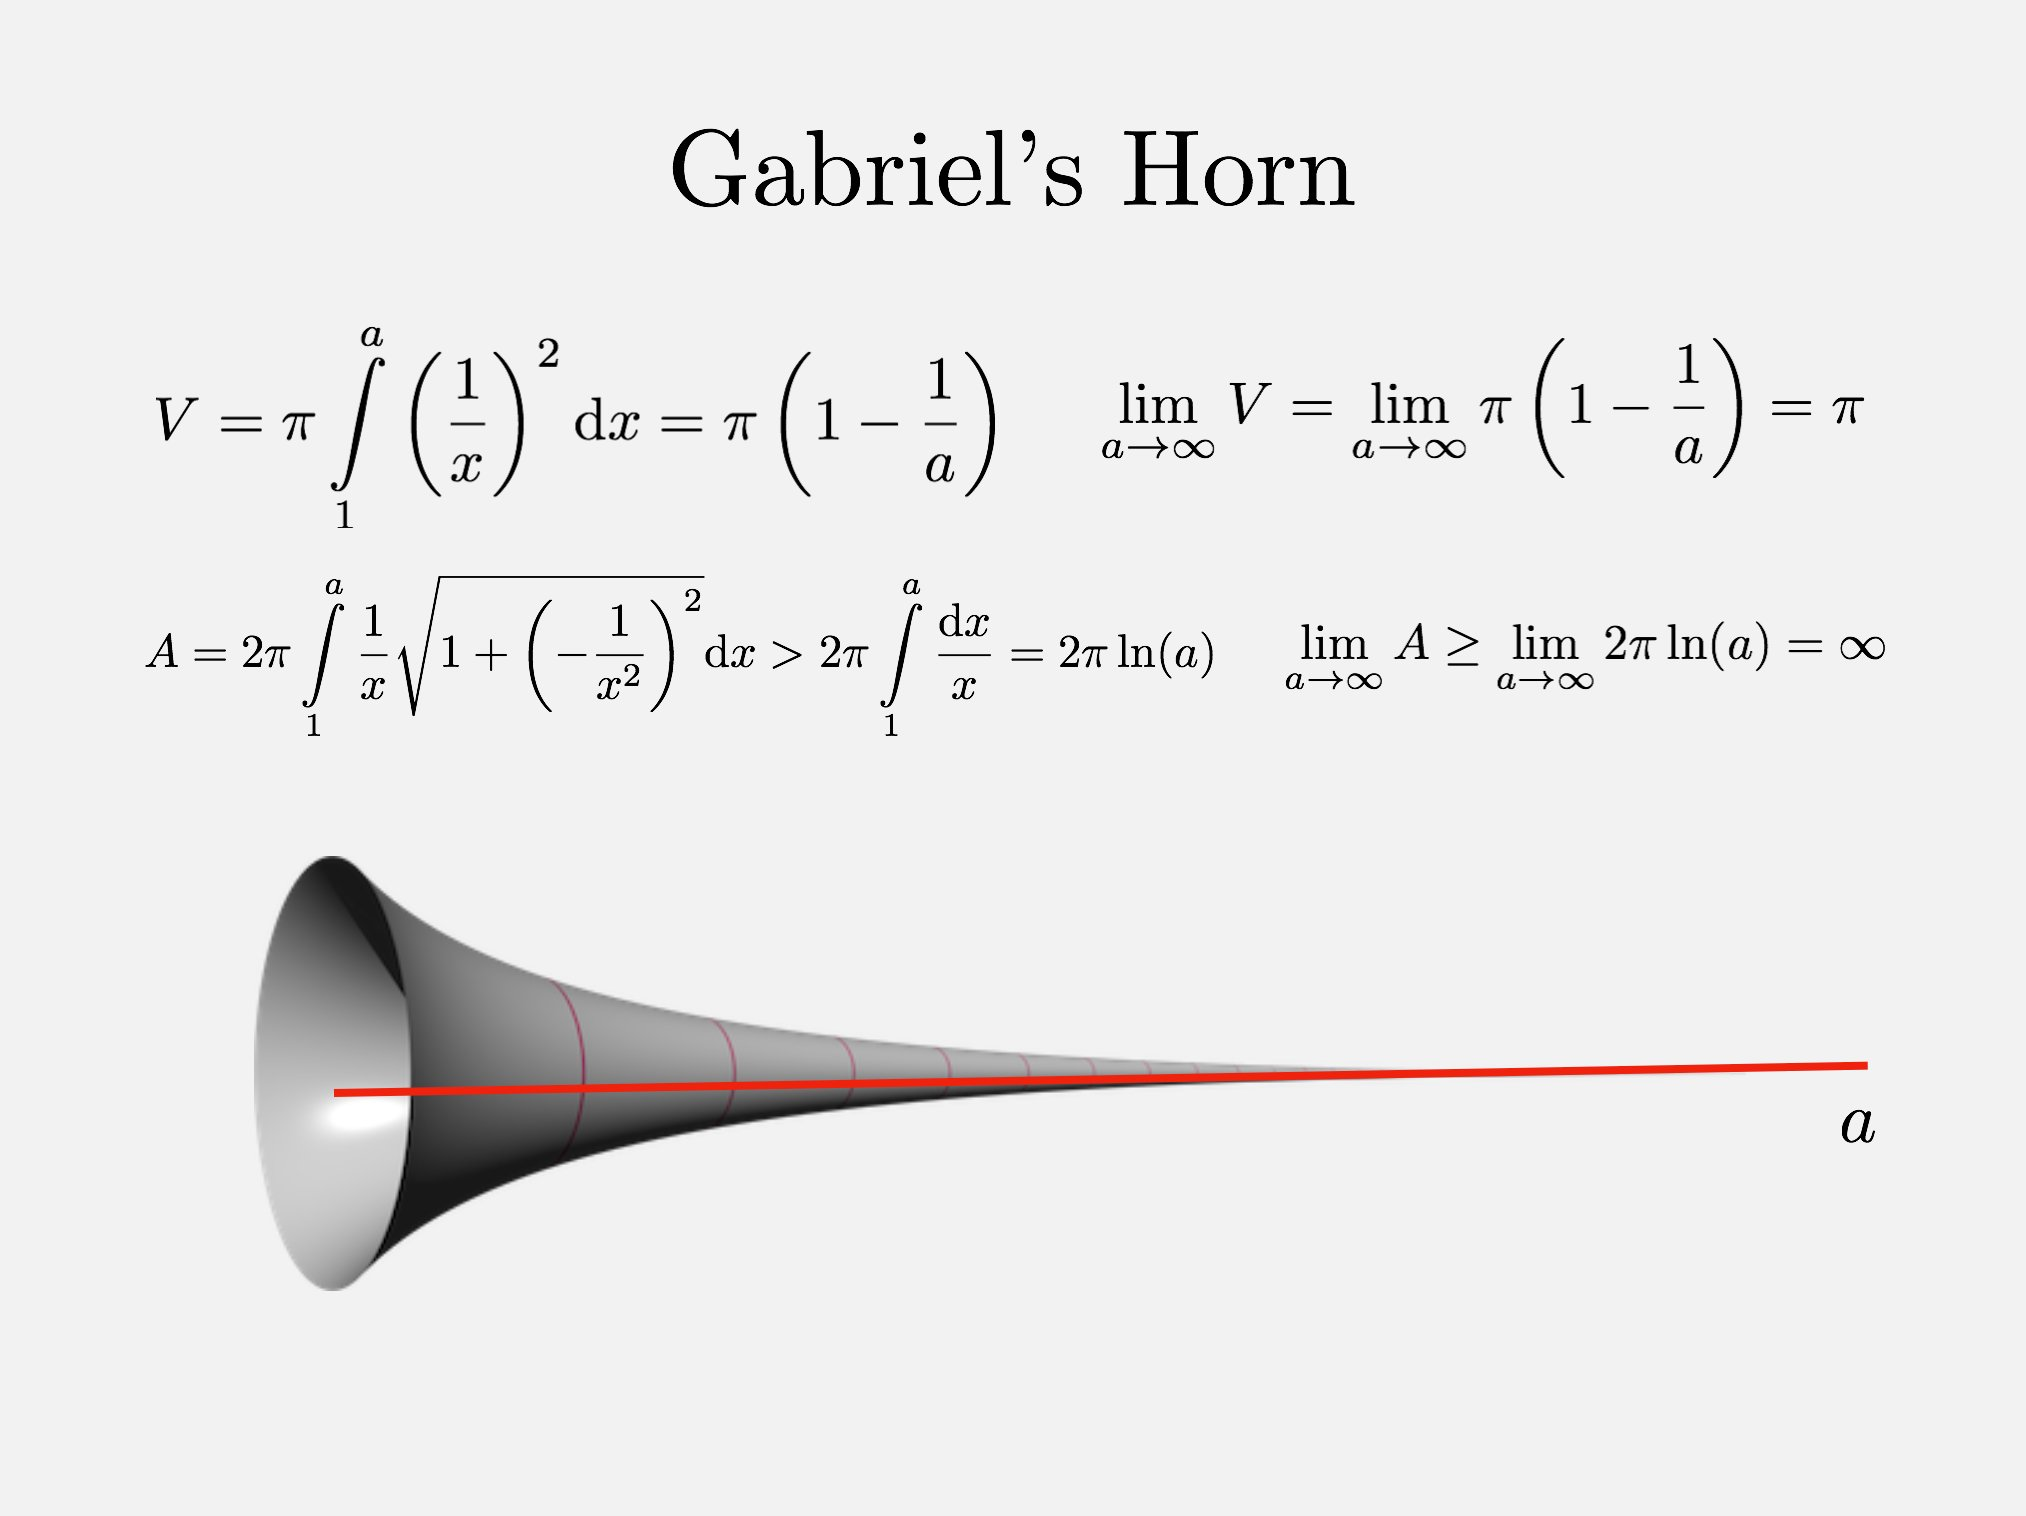
\includegraphics[frame, scale=0.15] {images/gabriels_horn.jpg}}
\caption{Gabriel's Horn}
\label{fig:gabriels_horn}
\end{figure}

\bigskip
\noindent
As we can see in Figure \ref{fig:gabriels_horn}, Gabriel's Horn
has volume $\pi$ and area $\infty$ in the limit. These properties
lead to an interesting situation known as the Painter's Paradox
\cite{painters_paradox_2,painters_paradox,painters_paradox_1}.
%
%
%
\subsection{The Painter's Paradox}
This is the Painter's Paradox: Somehow even though you can 
fill Gabriel's Horn with paint (its volume is finite), you 
still won't have enough paint to cover its inside surface 
(its area is infinite)!
%
%
%
\section{Fermat's Christmas Theorem}
%
%
%
\noindent
Fermat's Christmas Theorem (aka Fermat's theorem on sums of two
squares) is a beautiful and simple
theorem which states that an odd prime number $p$ can be
expressed as

\smallskip
\begin{center}
\scalebox{1.25} {$p = r^{2} + s^{2}$}
\end{center}

\smallskip
\noindent
where $r,s \in \mathbb{N}$, if and only if $p \equiv 1 \textrm{
(mod $4$)}$. That is, the theorem holds iff $p = 4n + 1$ for some
$n \in \mathbb{N}$ \cite{wiki:christmas_theorem}.

\bigskip
\noindent
For example, the primes 5, 13, 17, 29, 37 and 41 are all
congruent to 1 modulo 4 and can be expressed as sums of two
squares in the following ways:

\smallskip
\begin{equation*}
\begin{array}{rcll} 
5   &=& 1^{2} + 2^{2}   \\
13  &=& 2^{2} + 3^{2}   \\
17  &=& 1^{2} + 4^{2}   \\
29  &=& 2^{2} + 5^{2}   \\
37  &=& 1^{2} + 6^{2}   \\
41  &=& 4^{2} + 5^{2}
\end{array}
\end{equation*}


\bigskip
\noindent
On the other hand, the primes 3, 7, 11, 19, 23 and 31 are all
congruent to 3 modulo 4 and none of them can be expressed as the
sum of two squares. This is the easier part of the theorem since
it follows immediately from the observation that all squares are
congruent to 0 or 1 modulo 4.


\bigskip
\noindent
The prime numbers $p$ for which Fermat's Christmas Theorem is
true are called Pythagorean primes.  See
\cite{wiki:pythagorean_primes} for more on Pythagorean primes.

\bigskip
\noindent
BTW, this theorem is called Fermat's Christmas Theorem because
Fermat announced a proof of the theorem in a letter to Mersenne
dated December 25, 1640. And of course, Fermat didn't include a
proof in the letter.


\bigskip
\noindent
A variety of proofs of Fermat's Christmas Theorem can be found in
\cite{wiki:christmas_theorem_proofs}.
%
%
%
\section{The 12 Days of Christmas}
\label{sec:12_days_of_christmas}
The classic English Christmas carol "The Twelve Days of
Christmas" has all kinds of interesting mathematical
features. For example, it is an example of a \emph{cumulative
song}, in which the lyrics detail a series of increasingly
numerous gifts given to the speaker by their "true love" on each
of the twelve days of Christmas (the twelve days that make up the
Christmas season, starting with Christmas Day)
\cite{wikipedia:cumulative_song}. This cumulative property leads
to a bunch of interesting questions including "How many gifts are
given each day?" and "What is the total number of gifts given
during the 12 Days of Christmas?".

\bigskip
\noindent
In any event the carol's words were apparently first published in
England in the late $18^{\text{th}}$ century (and has a Roud Folk
Song Index number of 68 if you happen to be interested in that
kind of thing \cite{wikipedia:roud_folk_song_index}). A large
number of different melodies have been associated with the song,
of which the best known is derived from a 1909 arrangement of a
traditional folk melody by English composer Frederic Austin
\cite{wikipedia:twelve_days_of_christmas}.  There are twelve
verses, each describing a gift given by "my true love" on one of
the twelve days of Christmas. Suffice it to say that are many
variations in the lyrics. That said, the lyrics I'm using here
are from Frederic Austin's 1909 publication that established the
current form of the carol \cite{wikipedia:frederic_austin}.

\bigskip
\noindent
The first three verses of Austin's version of the carol are:

\smallskip
\begin{enumerate}
\item On the first day of Christmas my true love sent to me:
\emph{A partridge in a pear tree}.

\item On the second day of Christmas my true love sent to me:
\emph{Two turtle doves, and a partridge in a pear tree}.

\item On the third day of Christmas my true love sent to me:
\emph{Three French hens, two turtle doves, and a partridge in 
a pear tree}.
\end{enumerate}

\smallskip
\noindent
The subsequent verses follow the same pattern. The verses deal
with the next day where it adds one new gift and then repeats all
the earlier gifts. So each verse is one line longer than the
previous verse. The subsequent verses add

\vspace{0.375em}
 \begin{enumerate}
   \addtocounter{enumi}{3}                                                                      % set counter so next item is 4
   \item 4 calling birds
   \item 5 gold rings
   \item 6 geese a-laying
   \item 7 swans a-swimming
   \item 8 maids a-milking
   \item 9 ladies dancing
   \item 10 lords a-leaping
   \item 11 pipers piping
   \item 12 drummers drumming
 \end{enumerate}

\subsection{How many gifts are received each day and what is the total?}
The number of gifts received on day {\bf n} and the total number
of gifts received by (including) day {\bf n} are shown in the
following table $(1 \leq {\mathbf n} \leq 12)$:
%
%
%
\vspace{1.25em}
%
%
\renewcommand*{\arraystretch}{1.95}                                             				% get some extra space in the table
%
%
%
\begin{table}[H]
 \centering
 \scalebox{0.70}{
   \begin{tabular}{|c|c|c|} 
      \hline
       {\large \bf Day} & {\large \bf Gifts received on day n} 
                       & {\large \bf Total number of gifts received by day n} \\
       \hline
       \hline
       1  & {\bf \color{blue}{1}} & {\bf \color{red}{1}} \\
       \hline
       2  & 1+2={\bf \color{blue}{3}} & 1+3={\bf \color{red}{4}} \\
       \hline
       3  & 1+2+3={\bf \color{blue}{6}} & 1+3+6={\bf \color{red}{10}} \\
       \hline
       4  & 1+2+3+4={\bf \color{blue}{10}} & 1+3+6+10={\bf \color{red}{20}} \\
       \hline
       5  & 1+2+3+4+5={\bf \color{blue}{15}} & 1+3+6+10+15={\bf \color{red}{35}} \\
       \hline
       6  & 1+2+3+4+5+6={\bf \color{blue}{21}} & 1+3+6+10+15+21={\bf \color{red}{56}} \\
       \hline
       7  & 1+2+3+4+5+6+7={\bf \color{blue}{28}} & 1+3+6+10+15+21+28={\bf \color{red}{84}} \\
       \hline
       8  & 1+2+3+4+5+6+7+8={\bf \color{blue}{36}} & 1+3+6+10+15+21+28+36={\bf \color{red}{120}} \\
      \hline 
       9  & 1+2+3+4+5+6+7+8+9={\bf \color{blue}{45}} & 1+3+6+10+15+21+28+36+45={\bf \color{red}{165}} \\
      \hline
       10 & 1+2+3+4+5+6+7+8+9+10={\bf \color{blue}{55}} & 1+3+6+10+15+21+28+36+45+55={\bf \color{red}{220}} \\
      \hline
       11 & 1+2+3+4+5+6+7+8+9+10+11={\bf \color{blue}{66}} & 1+3+6+10+15+21+28+36+45+55+66={\bf \color{red}{286}} \\
      \hline
       12 & 1+2+3+4+5+6+7+8+9+10+11+12={\bf \color{blue}{78}} & 1+3+6+10+15+21+28+36+45+55+66+78={\bf \color{red}{364}} \\
      \hline
     \end{tabular}}
  \caption{Gift counts for the 12 days of Christmas}
  \label{tab:12_days_of_christmas}
\end{table}

\bigskip
\noindent
Interestingly, the numbers in blue in Table
\ref{tab:12_days_of_christmas}, the number of gifts received on
day {\bf n}, are called triangular numbers. Why? We will see in
Section \ref{subsec:geometric_interpretation} that there is an
interesting geometric interpretation that motivates this name.

\bigskip
\noindent
The $n^{\text{th}}$ triangular number, $T_{n}$, is defined as
follows:



\begin{equation}
T_{n}= \sum _{k=1}^{n} k = \frac {n(n+1)}{2} = {n+1 \choose 2}
\label{eqn:triangular_number}
\end{equation}


\noindent
where ${\displaystyle \binom{n}{m}}$ is the familiar binomial
coefficient\footnote{Aside: The great mathematician Carl
Friedrich Gauss is said to have discovered the consecutive
integer formula (Equation (\ref{eqn:triangular_number})) while
still at primary school \cite{gauss_day_of_reckoning}.}. For example,
$T_{12} = \sum\limits_{k=1}^{12} k = \frac{12 \cdot 13}{2} = {13
\choose 2} = \mathbf{\color{blue} 78}$.

\medskip
\noindent
So how many total gifts have been received by day {\bf n}?  If we
look at the {\bf Total number of gifts received by day n} column
of Table \ref{tab:12_days_of_christmas} we can see a pattern. In
particular, the number of gifts received by (including) day {\bf
n} is the sum of the gifts received on the previous days plus the
gifts received on day {\bf n}.  The number of gifts received by
day {\bf n} is shown in red in Table
\ref{tab:12_days_of_christmas}.  These numbers are called the
tetrahedral numbers and are defined as follows \cite{A000292}:


\begin{equation}
T_{e_n} = \sum\limits_{k=1}^{n} T_k = \frac{n(n+1)(n+2)}{6} = 
          \binom{n+2}{3}
\label{eqn:tetrahedral_number}
\end{equation}

\bigskip
\noindent
where $T_{k}$ is the $k^{\text{th}}$ triangular number 
(Equation (\ref{eqn:triangular_number})).

\vspace{0.74em}
\noindent
It turns out that the total number of gifts received by day 12,
$T_{e_{12}}$, is $\sum\limits_{k=1}^{12} T_k =\frac{12 \cdot 13
\cdot 14}{6} = \binom{14}{3} = \mathbf{\color{red} {364}}$.

% \bigskip
\noindent
BTW, can a number can be both triangular and tetrahedral? Well,
if so there would have to exist $m,n \in \mathbb{N}$ such
that


\bigskip
\begin{equation}
T_{n} = \binom{n+1}{2} = \binom{m+2}{3} = T_{e_m}
\label{eqn:triangular_and_tetrahedral}
\end{equation}

\vspace{1.5em}
\noindent
Apparently the only $m,n$ that satisfy Equation 
(\ref{eqn:triangular_and_tetrahedral})
are \cite{A027568}:

\medskip
\begin{equation*}
\begin{array}{llllll}
T_{e_1}    \; = T_{1}   \;\; = \; 1    \\
T_{e_3}    \; = T_{4}   \;\; = \; 10   \\
T_{e_8}    \; = T_{15}    \; = \; 120  \\
T_{e_{20}}    = T_{55}    \; = \; 1540 \\
T_{e_{34}}    = T_{119}      = \; 7140 
\end{array}
\end{equation*}

\vspace{0.25em}
\subsection{Pascal's triangle}
\label{subsec:pascals_triangle}
"The 12 Days of Christmas" also has interesting connections to
Pascal's triangle \cite{wiki:pascals_triangle}. Specifically, the
$3^{\text{rd}}$ diagonal of Pascal's triangle, shown in blue in
Figure \ref{fig:pascals_triangle}, contains the numbers we see in
{\bf Gifts received on day n} column of Table
\ref{tab:12_days_of_christmas}. These are the triangular numbers
(Equation (\ref{eqn:triangular_number})).  Similarly, the
$4^{\text{th}}$ diagonal of Pascal's triangle, shown in red in
Figure \ref{fig:pascals_triangle}, contains the {\bf Total number
of gifts received by day n} column of Table
\ref{tab:12_days_of_christmas}. These are the tetrahedral numbers
(Equation (\ref{eqn:tetrahedral_number})).

\vspace{1.5em}
%                                                                       % start building pascal's triangle
%       Parameters and settings                                         % start with the parameters and settings
%                                                                       %
\def \nrows {14}                                                        % number of rows in the triangle
\setlength {\fboxsep}{1em}                                              % get some more space around the \fbox	
%                                                                       %
%       Build the figure                                                % build the figure
%                                                                       %
\begin{figure}[H]                                                       % begin the figure
  \centering                                                            % center everything
  \fbox {                                                               % put a box around the figure
    \resizebox{0.725 \textwidth}{!} {                                   % resize the figure if you want
     \begin{mplibcode}                                                  % MetaPost...
        vardef Pascal_triangle(expr n, u, v) =                          % define the function
          save b; numeric b[][]; clearxy;                               % declare some variables
          defaultscale := 16pt/fontsize defaultfont;                    % set the font the way I want
          b[0][0] = 1; b[0][1] = 0; label("1", origin);                 % special case the "ones"
          for i = 1 upto n:                                             % loop over the rows
            x := -u*i/2; y := -i*v;                                     % draw the result at (x,y)
            b[i][0] = 1; label("1", z);                                 % need one more "one"
            for k = 1 upto i:                                           % loop over the columns
              x := x + u;                                               % compute the coordinates
              b[i][k] = b[i-1][k-1] + b[i-1][k];                        % compute the value of the binomial
              if k = 2:                                                 % triangular numbers
                label(decimal(b[i][k]),z) withcolor blue;               % triangular numbers in blue
              elseif k = 3:                                             % tetrahedral numbers
                label(decimal(b[i][k]),z) withcolor red;                % tetrahedral numbers in red
              else:                                                     % default
                label(decimal(b[i][k]),z) withcolor black;              % default to black
              fi                                                        % end else
            endfor                                                      % end for
            b[i][i+1] = 0;                                              % 
          endfor                                                        %
        enddef;                                                         %
%                                                                       %
%       Draw the triangle                                               %
%                                                                       %
        beginfig(1);                                                    % draw the triangle
          Pascal_triangle(\nrows, 1.4cm, 1cm);                          % draw \nrows
        endfig;                                                         %
     \end{mplibcode}                                                    %
     }                                                                  % end resizebox
  }                                                                     % end fbox
  \caption{Pascal's triangle with the triangular numbers in             % caption the figure
           blue and the tetrahedral numbers in red}						% caption the figure.2
  \label{fig:pascals_triangle}                                          % label the figure
\end{figure}                                                            % end figure


\noindent
Pascal's triangle can also be drawn with binomial coefficients.
This is shown is Figure \ref{fig:pascals_triangle_with_binomial_coefficients}
with the triangular numbers in blue and the tetrahedral numbers in red.

\vspace{1.25em}
%
%       Parameters
%
\def \nrows {14}                                                 		% number of rows
%
%
%	Draw the picture
%
\begin{figure}[H]                                                       % build the triangle
  \centering                                                            % center everything
   \resizebox{0.55 \textwidth}{!} {                                     % resize the figure if you want
    \begin{tikzpicture} [framed,scale=0.90]                             % put a frame on the tikzpicture 
       \foreach \n in {0,...,\nrows} {                                  % iterate over rows
          \foreach \k in {0,...,\n} {                                   % iterate over columns
             \node at (\k-\n/2,-\n) {                                   % put the coefficient here
             \ifnum \k = 2 {\color{blue} ${\binom{\n}{\k}}$}            % k = 2 => triangular number
                \else                                                   % else
                  \ifnum \k = 3 {\color{red}${\binom{\n}{\k}}$}         % k =3 => tetrahedral number
                    \else {\color{black}${\binom{\n}{\k}}$}             % default to black
                   \fi                                                  % end \ifnum \k = 3
              \fi};                                                     % end \ifnum \k = 2
          }                                                             % end \foreach \k ...
        }                                                               % end \foreach \n ...
    \end{tikzpicture}                                                   % end tikzpicture
   }                                                                    % end resizebox
  \caption{Pascal's triangle with binomial coefficients}
  \label{fig:pascals_triangle_with_binomial_coefficients}
\end{figure}

\smallskip
\subsection{Geometric interpretations}
\label{subsec:geometric_interpretation}
There are interesting geometric interpretations of both the
triangular and tetrahedral numbers. So first, what exactly is a
triangular number?  The first six triangular numbers are depicted
as triangles in Figure \ref{fig:triangular_numbers}.  We can see
from the figure that the $n^{\text{th}}$ triangular number, $T_n$,
is the sum of the integers from 1 to $n$ \cite{wiki:triangle_numbers}.  
This is the number of gifts received on the $n^{\text{th}}$ day of
Christmas according to "The 12 Days of Christmas".
  
\vspace{1.05em}
\begin{figure}[H]
  \center{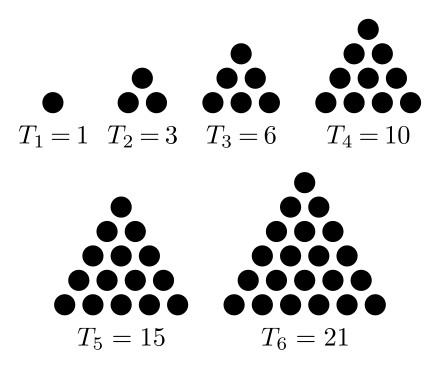
\includegraphics[frame,scale=0.35]
         {images/first_six_triangular_numbers.png}} 
  \caption{The first six triangular numbers}
  \label{fig:triangular_numbers}
\end{figure}


\noindent
Ok, then what are the tetrahedral numbers? As we saw in Equation
(\ref{eqn:tetrahedral_number}), the $n^{\text{th}}$ tetrahedral
number is the sum of the first $n$ triangular numbers
\cite{wolfram:tetrahedral_numbers}. If we stack up these
triangular numbers we get a tetrahedron (hence the name
"tetrahedral number"). For example, $T_{e_{4}}$ is depicted in
Figure \ref{fig:tetrahedral_numbers}. The $n^{\text{th}}$
tetrahedral number turns out to be the number of gifts received
up to and including day {\bf n} in "The 12 Days of Christmas".
%
%
%
%\vspace{1.0em}
\begin{figure}[H]
  \center{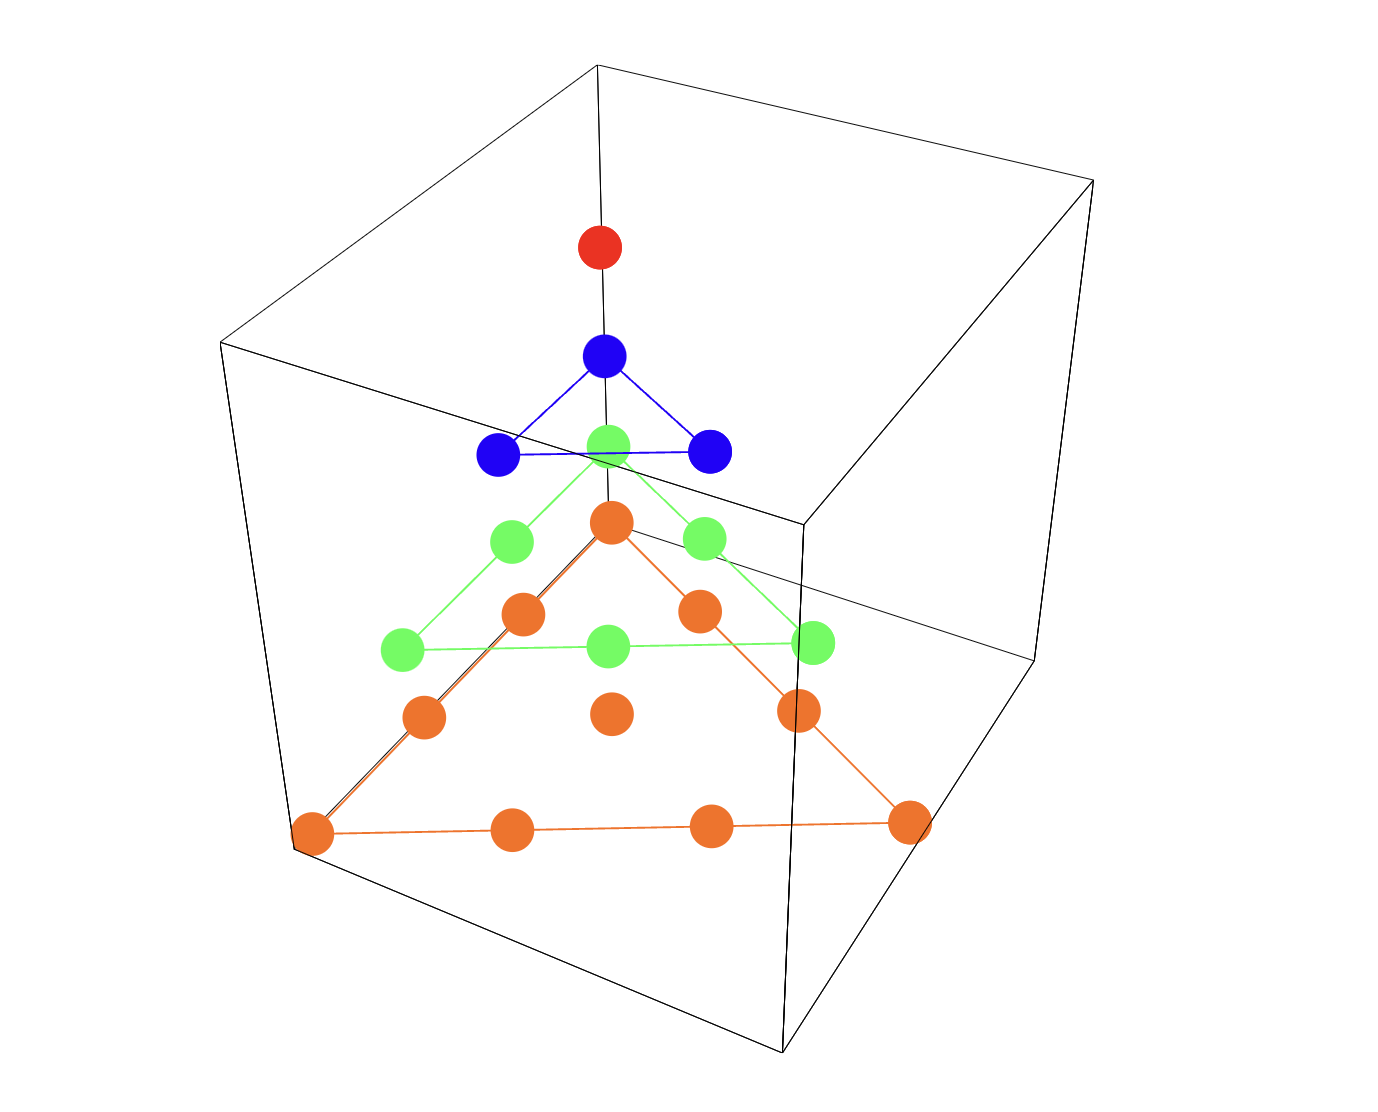
\includegraphics[frame,scale=0.25]
                          {images/tetrahedral_numbers.png}} 
  \caption{The fourth tetrahedral number $T_{e_{4}} = 20$}
  \label{fig:tetrahedral_numbers}
\end{figure}
%
%
%
\section{The Christmas Stocking Theorem}
"The Christmas stocking theorem, also known as the hockey stick
theorem, states that the sum of a diagonal string of numbers in
Pascal's triangle starting at the nth entry from the top (where
the apex has $n = 0$) on left edge and continuing down $k$ rows
is equal to the number to the left and below (the "toe") bottom
of the diagonal (the "heel"; Butterworth 2002)."
\cite{christmas_stocking_theorem}.

\bigskip
\noindent
That is, Christmas Stocking Theorem states that for all $n \in
\mathbb{N}$ we have

\medskip
\begin{equation*}
\sum\limits_{i=0}^{k-1} {n+i \choose i} = {k+n \choose k-1}
\end{equation*}

\smallskip
{\setstretch{1.75}
\noindent
where ${\displaystyle {n \choose k}}$ is a binomial coefficient
(aka "$n$ choose $k$") \cite{wiki:binomial_coefficient}. This
is shown in Figure
\ref{fig:christmas_stocking_theorem}.  \par}


\vspace{1.25em}
\begin{figure} [H]
  \center{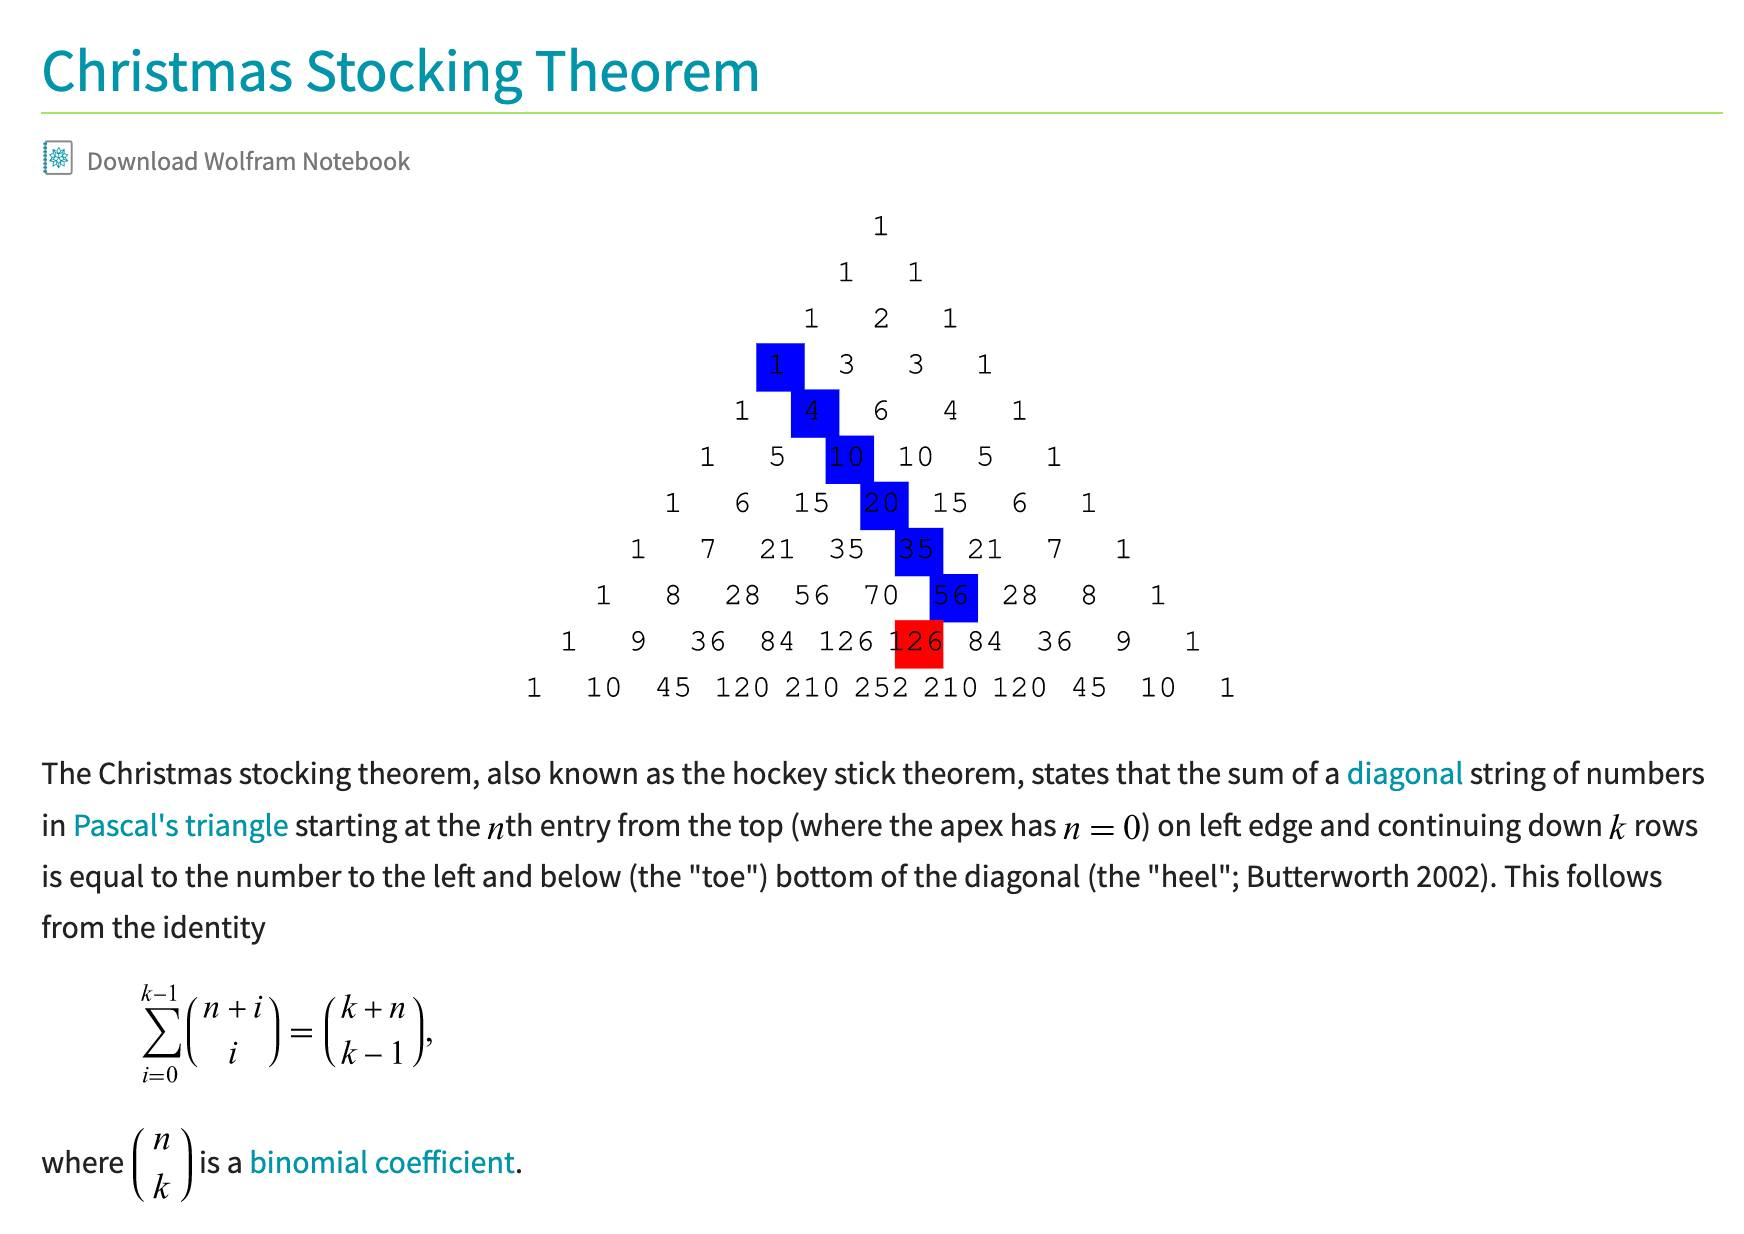
\includegraphics[frame, scale=0.20] {images/christmas_stocking_theorem.jpg}}
  \caption{The Christmas Stocking Theorem}
  \label{fig:christmas_stocking_theorem}
\end{figure}

\section{The Hitomezashi Christmas Tree}
A randomly generated "Christmas tree" filled with 
Hitomezashi pattern in 3 directions, one for each side,
is shown in Figure \ref{figure:hitomezashi_christmas_tree}
(image credit: @lambda@vis.social).

\bigskip
\noindent
What is a Hitomezashi pattern?

\bigskip
\noindent
Sashiko is a Japanese style of embroidery that developed during the Edo 
period (1603–1867) for both practical and decorative purposes. Its name, 
which translates to “little stabs,” refers to the act of stabbing a 
needle through cloth. One type of sashiko artwork known as hitomezashi 
(translating to “one-stitch”) uses simple rules to create beautiful 
geometric patterns in a rectangular grid \cite{hitomezashi_stich_pattern,
hitomezashi_pattern,mathematical_specification_of_hitomezashi_designs}.


\bigskip
\begin{figure} [H]
  \center{\fcolorbox{red}{white}{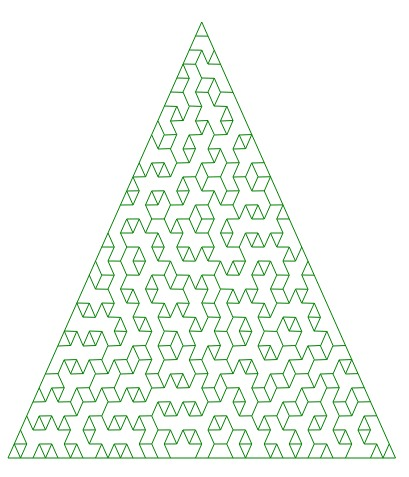
\includegraphics[scale=0.455] {images/hitomezashi_christmas_tree.jpg}}}
  \caption{Hitomezashi Christmas Tree}
  \label{figure:hitomezashi_christmas_tree}
\end{figure}


\smallskip
\section{Just For (More) Fun}

\setlength {\fboxsep} {0.85em}											% get more space between fcolorbox and content
\setlength {\fboxrule}{0.75pt}											% change fcolorbox line thickness

\begin{figure} [H]
  \centering                                                            % center everything
  \fcolorbox{red}{white} {                                            	% put a color box around the figure
    \resizebox{0.70 \textwidth}{!} {                                     % resize the figure if you want
       \begin{math}
          \begin{array}{rcll} 
             y
             &\coloneqq& {\displaystyle \frac{\ln \big (\frac{x}{m} -  sa  \big ) }{r^2}}
                         &\qquad \qquad \mathrel{\#} \text{define $y$} \\
[1pt]
             &\Rightarrow& r^2 y = \ln \big (\frac{x}{m} -  sa  \big )    
                         &\qquad \qquad  \mathrel{\#} \text{multiply both sides on the left by $r^2$} \\
[1pt]
             &\Rightarrow& e^{r^2y} = e^{\ln \big ( \frac{x}{m} -  sa\big )}                           
                         &\qquad \qquad \mathrel{\#} \text{$x = y \Rightarrow b^x =b^y$ ; exponentiate with $b = e$} \\
[1pt]
             &\Rightarrow& e^{r^2y} = \frac{x}{m} -  sa                           
                         &\qquad \qquad \mathrel{\#} e^{\ln(x)} = x \\
[1pt]
             &\Rightarrow& e^{r^2y} = \frac{x}{m} -  as						
                         &\qquad \qquad \mathrel{\#} \text{assume multiplication is commutative $(sa = as)$} \\ 
[1pt]
             &\Rightarrow& m e^{r^2y} = x - mas                                        
                         &\qquad \qquad \mathrel{\#} \text{multiply both sides on the left by $m$} \\
[1pt]
             &\Rightarrow& \bf{\color{red}{m e^{rry} = x - mas}}                                     
                         &\qquad \qquad \mathrel{\#} \text{$r^2 = rr \Rightarrow$ \bf{Merry X-mas!}}
         \end{array}
       \end{math}
        }                                                               % end resizebox
     }                                                                  % end fcolorbox
  \caption{Merry Christmas Everyone!}
  \label{fig:merry_christmas_everyone}
\end{figure}
%
%
%
\section*{Acknowledgements}
\label{sec:acknowledgements}
Special thanks to Alice Meyer for suggesting that I collect my
"Christmastime is Christmas Math Time!" examples in one document.
%
%	LaTeX source on overleaf.com
%
\section*{\LaTeX \hspace{0.10 mm} Source}
\url{https://www.overleaf.com/read/fwsfybtfmryr}
%
%	get a bibliography
%
%	Note:.bib files go in ~/Library/texmf/bibtex/bib with TeXShop (MacTeX).
%	You can also use an absolute path, e.g. \bibliography{/Users/dmm/papers/bib/qc}
%
\bibliographystyle{plain}
\bibliography{qc}
%
%	done
%
\end{document} 

